\documentclass[12pt,letterpaper]{article}
\usepackage[margin=.63in,headheight=16pt,headsep=.18in,footskip=.26in]{geometry}
\usepackage[T1]{fontenc}
\usepackage[scaled=.95]{helvet}
\renewcommand{\familydefault}{\sfdefault}
\usepackage{tikz,array,fancyhdr,amsmath}
\usetikzlibrary{arrows.meta}
\definecolor{ink}{RGB}{33,39,45}
\definecolor{blue}{RGB}{32,91,137}
\definecolor{ballgray}{RGB}{249,250,250}
\color{ink}
\pdfinfoomitdate=1
\pdftrailerid{}
\pdfsuppressptexinfo=15
\pagestyle{fancy}\fancyhf{}
\renewcommand{\headrulewidth}{.35pt}
\renewcommand{\footrulewidth}{.25pt}
\fancyfoot[L]{\scriptsize Bellingham Math Circle / Week 61 / W61-S-v2}
\fancyfoot[R]{\scriptsize\thepage}
\newcommand{\band}[1]{\fancyhead[L]{\small Week 61 / Triangles on a ball / Grades #1}}
\setlength{\parindent}{0pt}\setlength{\parskip}{8pt}
\newcommand{\problem}[2]{\textbf{Problem #1:} #2\par}
\newcommand{\writing}[1]{\vspace{2pt}\begin{tikzpicture}[x=1in,y=1in]\foreach \y in {1,...,#1}{\draw[ink!25] (0,-.43*\y) -- (6.95,-.43*\y);}\end{tikzpicture}\par}
\newcommand{\sphereblank}{\begin{tikzpicture}[x=1in,y=1in]\path[use as bounding box] (-1.38,-1.40) rectangle (1.38,1.40);\draw[ink!60] (0,0) circle (1.18);\end{tikzpicture}}
\newcommand{\recordblank}{\begin{tikzpicture}[x=1in,y=1in]\path[use as bounding box] (-1.28,-1.08) rectangle (1.28,1.08);\draw[ink!60] (0,0) circle (.98);\end{tikzpicture}}
\input{figures.tex}
\begin{document}
\band{2--5}
Keep the ball on its support. Keep the string against its surface and its endpoints on the same two markers. Dashed arcs lie on the back of the ball.

A \textit{great circle} is the circle made by a flat cut through the ball's center. For two distinct points that are not opposite, its shorter arc is the shortest surface route.

\begin{center}
\begin{tabular}{ccc}
\routeinput & \routecircle & \routeoutput\\[-1pt]
\small Mark $P$ and $Q$ & \small Their great circle & \small Shorter arc: $P$ to $Q$
\end{tabular}
\end{center}

\problem{1}{Choose a close pair of markers, a far-apart pair that is not opposite, and a pair exactly opposite each other on your ball. Find the shortest surface routes for each pair. Which pairs let you find two different routes of the same shortest length? Draw your routes.}

\begin{center}\begin{tabular}{ccc}
\small Close pair & \small Far-apart pair & \small Opposite pair\\
\begin{tikzpicture}[x=.82in,y=.82in]\draw[ink!60] (0,0) circle (1);\path[use as bounding box] (-1.25,-1.15) rectangle (1.25,1.15);\end{tikzpicture}&
\begin{tikzpicture}[x=.82in,y=.82in]\draw[ink!60] (0,0) circle (1);\path[use as bounding box] (-1.25,-1.15) rectangle (1.25,1.15);\end{tikzpicture}&
\begin{tikzpicture}[x=.82in,y=.82in]\draw[ink!60] (0,0) circle (1);\path[use as bounding box] (-1.25,-1.15) rectangle (1.25,1.15);\end{tikzpicture}
\end{tabular}\end{center}
\writing{3}

\newpage\band{2--5}
Our triangles enclose some surface area, with three distinct corners and shortest great-circle arcs. No two corners are opposite. Use the smaller convex region: each inside corner is less than $180^\circ$, and the whole triangle fits strictly inside an open half of the ball.

An angle on the ball is the angle between the directions of the two sides at their meeting point. Use the inside corner. A flat picture of the ball is a sketch, not an angle meter.

\begin{center}\begin{tabular}{ccc}
\angleinput &
\begin{tikzpicture}[x=.7in,y=.7in]\path[use as bounding box] (-1.1,-1.1) rectangle (1.1,1.1);\draw[blue,line width=1.5pt] (0,0)--(.9,0);\draw[blue,line width=1.5pt] (0,0)--(135:.9);\draw[ink] (.28,0) arc (0:135:.28);\node[font=\small] at (62:.55) {$135^\circ$};\fill[ink] (0,0) circle (.025);\node[font=\small,anchor=north] at (0,-.05) {$P$};\end{tikzpicture}&
\begin{tikzpicture}[x=.7in,y=.7in]\path[use as bounding box] (-1.1,-1.1) rectangle (1.1,1.1);\draw[ink!40] (-.85,-.4) rectangle (.85,.4);\node[font=\small] at (0,0) {$P:\ 135^\circ$};\end{tikzpicture}\\[-1pt]
\small Two sides at $P$ & \small Directions close to $P$ & \small Angle record
\end{tabular}\end{center}

\problem{2}{Make a triangle on your ball with as many right-angle corners as you can. Check its corners with the paper right angle. Can all three corners be right angles? Draw your best triangle and mark its corners.}

\begin{center}\sphereblank\end{center}
\writing{3}

\newpage\band{2--5}
The equator is a great circle. $N$ is the pole above it. A meridian is a great-circle semicircle from $N$ to the opposite pole. Its corner with the equator is a right angle.

\problem{3}{Keep $N$ fixed. Move $A$ and $B$ on the equator, using its shorter arc as the third side. Make triangles whose corner at $N$ is smaller than a right angle, equal to a right angle, and larger than a right angle. Draw each triangle and mark all its corners. Which changes make the triangle cover more of the ball?}

\begin{center}\movingtriangle\end{center}

\begin{center}\begin{tabular}{cc}
\small $N$ corner smaller than a right angle & \small $N$ corner equal to a right angle\\
\recordblank & \recordblank
\end{tabular}\end{center}
\begin{center}\begin{tabular}{cc}
\small $N$ corner larger than a right angle & \small Extra workspace\\
\recordblank & \recordblank
\end{tabular}\end{center}

\newpage\band{3--5}
A \textit{lune} is the strip between two great-circle semicircles from $N$ to its opposite pole $S$. The strip's angle is the gap between them at $N$. Fractions refer to the ball's surface.

\begin{center}\begin{tabular}{ccc}
\luneexample &
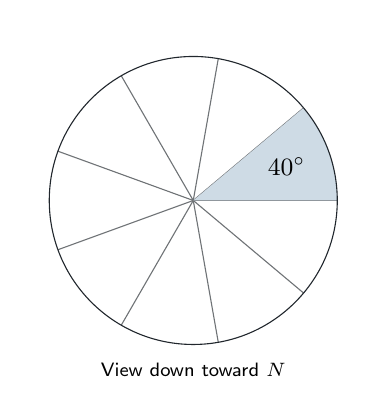
\begin{tikzpicture}[x=.72in,y=.72in]\path[use as bounding box] (-1.15,-1.2) rectangle (1.15,1.2);\foreach \a in {0,40,...,320}{\draw[ink!65] (0,0)--(\a:1);}\fill[blue!22] (0,0)--(0:1) arc (0:40:1)--cycle;\draw[ink] (0,0) circle (1);\node[font=\small] at (20:.69) {$40^\circ$};\node[font=\scriptsize,anchor=north] at (0,-1.06) {View down toward $N$};\end{tikzpicture}&
\begin{tikzpicture}[x=.72in,y=.72in]\path[use as bounding box] (-1.15,-1.2) rectangle (1.15,1.2);\node[font=\normalsize] at (0,.18) {$360\div40=9$};\node[font=\normalsize] at (0,-.28) {One lune: $\frac19$ of the surface};\end{tikzpicture}\\
\small $40^\circ$ lune & \small 9 equal lunes fill the ball & \small Area record
\end{tabular}\end{center}

\problem{4}{Use the marked meridian pairs with gaps $45^\circ$, $72^\circ$, and $120^\circ$. For each pair, make a triangle with $N$ and the two equator points. What fraction of the ball's surface does each triangle cover?}

\begin{center}\begin{tabular}{>{\centering\arraybackslash}p{1.55in}|>{\centering\arraybackslash}p{1.55in}|>{\centering\arraybackslash}p{1.55in}}
$45^\circ$ gap & $72^\circ$ gap & $120^\circ$ gap\\[6pt]
\begin{tikzpicture}[x=.67in,y=.67in]\draw[ink!60] (0,0) circle (1);\path[use as bounding box] (-1.1,-1.1) rectangle (1.1,1.1);\end{tikzpicture}&
\begin{tikzpicture}[x=.67in,y=.67in]\draw[ink!60] (0,0) circle (1);\path[use as bounding box] (-1.1,-1.1) rectangle (1.1,1.1);\end{tikzpicture}&
\begin{tikzpicture}[x=.67in,y=.67in]\draw[ink!60] (0,0) circle (1);\path[use as bounding box] (-1.1,-1.1) rectangle (1.1,1.1);\end{tikzpicture}\\[22pt]
Fraction: \rule{.8in}{.3pt}&Fraction: \rule{.8in}{.3pt}&Fraction: \rule{.8in}{.3pt}\\[8pt]
\end{tabular}\end{center}
\writing{6}

\newpage\band{4--5}
At a triangle corner, extend its two meeting sides to full great circles. Choose the lune containing the triangle and the opposite lune. Together they are a \textit{lune pair}. A starred point is exactly opposite its matching letter.

\begin{center}\begin{tabular}{cccc}
\pairinput & \paircircles & \pairfront & \pairback\\[-2pt]
\small Corner $A$ & \small Circles $AB$ and $AC$ & \small Pair at $A$: front & \small Same pair: back
\end{tabular}\end{center}
\begin{center}\renewcommand{\arraystretch}{1.05}\begin{tabular}{c|c|c}
Marked pair & Patch & Count\\\hline
$A$ & $X$ & $1$
\end{tabular}\end{center}
Each pair covers a patch once or not at all. Front and back show the same ball; these views omit hidden arcs.

\problem{5}{Use a triangle with three right angles on your ball. Extend its sides to full great circles. For each of its three corners, mark the lune pair. How many of the three pairs cover each of the eight regions? Use your counts to explain what fraction of the ball the triangle covers.}

\begin{center}\begin{tabular}{cc}
\countfront & \countback\\[-4pt]
\small Front & \small Back
\end{tabular}\end{center}
\begin{center}\renewcommand{\arraystretch}{1.45}\begin{tabular}{c|cccccccc}
Region & 1&2&3&4&5&6&7&8\\\hline
Pairs covering it & \rule{.30in}{.3pt}&\rule{.30in}{.3pt}&\rule{.30in}{.3pt}&\rule{.30in}{.3pt}&\rule{.30in}{.3pt}&\rule{.30in}{.3pt}&\rule{.30in}{.3pt}&\rule{.30in}{.3pt}
\end{tabular}\end{center}
\writing{2}

\newpage\band{4--5}
\problem{6}{The triangle $ABC$ has three $80^\circ$ surface corners. Use these views to mark which pairs, at $A$, $B$, and $C$, cover each region. Do the unequal regions give the same counts as Problem 5? Use the pair areas and your counts to find the triangle's fraction of the ball.}

\begin{center}\begin{tabular}{cc}
\unequalfront & \unequalback\\[-2pt]
\small Front & \small Back
\end{tabular}\end{center}

\begin{center}\renewcommand{\arraystretch}{1.9}\begin{tabular}{c|cccccccc}
Region & 1&2&3&4&5&6&7&8\\\hline
Pair letters & \rule{.38in}{.3pt}&\rule{.38in}{.3pt}&\rule{.38in}{.3pt}&\rule{.38in}{.3pt}&\rule{.38in}{.3pt}&\rule{.38in}{.3pt}&\rule{.38in}{.3pt}&\rule{.38in}{.3pt}\\
Count & \rule{.38in}{.3pt}&\rule{.38in}{.3pt}&\rule{.38in}{.3pt}&\rule{.38in}{.3pt}&\rule{.38in}{.3pt}&\rule{.38in}{.3pt}&\rule{.38in}{.3pt}&\rule{.38in}{.3pt}
\end{tabular}\end{center}
\writing{7}

\newpage\band{4--5}
\problem{7}{Find a rule for a triangle's fraction of the ball using the sum of its three surface corners. Explain why the covering counts persist for every triangle under our rules, and why opposite triangles have equal area. Use your rule for these three exact surface-angle records.}

\begin{center}\begin{tabular}{ccc}
\recorda & \recordb & \recordc\\[-1pt]
\small $A=60^\circ,\ B=60^\circ,\ C=90^\circ$ & \small $A=B=C=80^\circ$ & \small $A=B=C=100^\circ$\\[18pt]
Fraction: \rule{1.0in}{.3pt} & Fraction: \rule{1.0in}{.3pt} & Fraction: \rule{1.0in}{.3pt}
\end{tabular}\end{center}
\writing{11}
\end{document}
